\section{Tools in MFE}
\label{sec.tools}

Five formal analysis tools are available 
in the current release of MFE.
The Maude Termination Tool (MTT) can be used
to prove termination of functional and
system modules, the Church-Rosser Checker (CRC)
can be used to check the Church-Rosser property 
of functional modules, the Coherence Checker (ChC)
can be used to check the coherence of system modules,
the Inductive Theorem Prover (ITP) can be used to verify 
inductive properties of functional modules, and
the Sufficient Completeness Checker (SCC) can
be used to check completeness of functional modules
and deadlock freedom of system modules.
One important aspect in the integration task
is the interaction complexity due to the nontrivial 
dependencies among tools. Figure~\ref{fig.tool-dep}
depicts the tool-dependency graph for these five tools.

\begin{figure}[htbp]
\begin{center}
%\fbox{
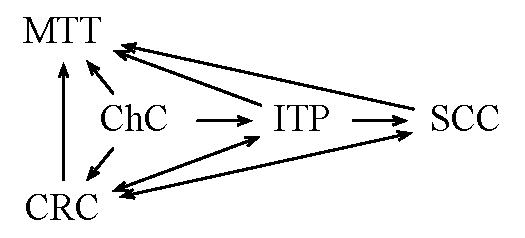
\includegraphics[width=5cm]{tool-dep}
%}
\caption{Tool-dependency graph in MFE.}
\label{fig.tool-dep}
\end{center}
\end{figure}

In the following paragraphs 
we summarize the main features
and dependencies of the five tools available in MFE. 
For further details on these tools, including user
manuals, restrictions, and examples, we refer the reader
to the given references and web sites.

\subsection{The Maude Termination Tool}
\label{sec.mtt}


Maude has expressive features including advanced typing constructs
with sorts, subsorts, kinds, and memberships; matching modulo axioms;
evaluation strategies for both equations and rewrite rules; and very 
general conditional equations and rewrite rules. Proving termination
of programs having such features is nontrivial. Furthermore, some of
these features are not supported by standard termination methods and
tools. Yet, the use of such features may be essential to ensure termination.
MTT uses several non-termination preserving theory 
transformations~\cite{Duran-Lucas-Meseguer:2009-prole,Duran-Lucas-Meseguer:2009-frocos}
which are applied in a kind of pipeline to a module $M$, obtaining
a module $M'$ in such a way that a proof termination of 
$M'$ witnesses the termination of $M$. For instance, 
by sequentially using four theory transformations,
a conditional order-sorted context-sensitive system module 
can be transformed into an unconditional unsorted
context-sensitive term rewrite system, which can be 
handled by the back-end tools.

The Maude Termination Tool (MTT) is a tool that checks the
termination of (possibly conditional) order-sorted
Maude functional or system modules. 
The current implementation takes a module
as input and tries to prove its termination by applying 
{theory transformations} and then invoking back-end termination tools,
such as MU-TERM~\cite{Lucas:2004} and AProVE~\cite{Giesl-Schneider-Kamp-Thiemann:2006}, that can prove termination of (variants of) rewriting.
For the current version of MFE, a new ``hook'' to a C++
library was included in non-official distribution of
Core Maude for invoking these back-end termination tools.
MTT is the only tool in the MFE
that does not depend on any other tool in the environment.

A stand-alone version of MTT, with a graphical user interface,
is available from \url{http://www.lcc.uma.es/~duran/MTT/}.

\subsection{The Church-Rosser Checker}
\label{sec.crc}

The Church-Rosser Checker (CRC) checks the
Church-Rosser property of Maude functional (possibly conditional)
order-sorted modules. For order-sorted modules, being Church-Rosser
and terminating means not only confluence, but also a 
{sort-decreasingness} property: each normal form has the least possible
sort among those of all equivalent terms.
CRC depends on MTT for checking termination assumptions
and on ITP for inductive theorem proving (see Section~\ref{sec.itp}).
Some of the proof obligations are not currently 
handled by any tool. We will se in Section~\ref{sec.example} that 
although they are submitted to ITP, these proofs may be ``trusted'' by the user.

CRC can be used to check equational specifications 
$(\Sigma,E\cup Ax)$ with an initial semantics that have already 
been proved terminating and need to be checked
(ground) Church-Rosser. The tool performs both a local confluence check
by computing all {\em (conditional) critical pairs} of the equations $E$
modulo the structural axioms $Ax$ 
%(i.e., overlaps among the left-hand sides of the equations in $E$ modulo $Ax$)
and a sort-decreasingness test in the form of membership assertions
for each equation in $E$ modulo $Ax$. If the 
(conditional) critical pairs or the sort decreasingness tests cannot
be discharged by CRC, proof obligations 
%consisting of a set of critical
%pairs and set of membership assertions that must be proven, respectively,
%(ground) joinable and (ground) reachable to a term with the required sort, 
are displayed as a guide to the user. In MFE, CRC can submit these
proof obligations to ITP for inductive
reasoning. 
%In other cases, the user may in
%fact have to modify the original specification by carefully considering the
%information conveyed by the proof obligations.

CRC, with its documentation and some examples, is available from
\url{http://maude.lcc.uma.es/CRChC/}.

\subsection{The Coherence Checker}
\label{sec.chc}

{\em (Ground) coherence} allows reducing the problem of computing rewrites of
the form $[t]_{E\cup Ax} \rews [t']_{E\cup Ax}$ that in general is
undecidable, to the much simpler and decidable problem of computing
rewrites of the form $[t]_{Ax} \rews [t']_{Ax}$, for $t$ and $t'$ 
any (ground) $\Sigma$-terms.
Intuitively, coherence means
that rewriting with $R$ modulo $E\cup Ax$ can be achieved by adopting
the strategy of first simplifying to canonical form with $E$ modulo $Ax$
and then applying a rule in $R$ modulo $Ax$.

The Coherence Checker (ChC) is a tool that provides a
(ground) coherence decision procedure for order-sorted system modules
$\rcal = (\Sigma,E\cup Ax,R)$. The tool calculates the set of
critical pairs between the equations $E$ and the rewrite rules $R$
modulo the structural axioms $Ax$, 
whose equational validity guarantees the (ground)
coherence of $\rcal$. ChC depends on MTT for termination
assumptions and on CRC for the equations $E$ being Church-Rosser.
Since this property is inductive, in some cases ITP can be used to
prove some proof obligations.

ChC, with its documentation and some examples, is available from
\url{http://maude.lcc.uma.es/CRChC/}.

\subsection{The Sufficient Completeness Checker}
\label{sec.scc}

Maude Sufficient Completeness Checker (SCC) is a tree automata based tool
for checking {\em sufficient completeness} and {\em deadlock
freedom} of terminating and sort-decreasing Maude modules.
Both sufficient completeness and deadlock freedom are relative
to {\em constructor} subsignatures.
For $\rcal=(\Sigma,E,R)$, a signature pair $(\Upsilon,\Omega)$,
with $\Upsilon \subseteq \Omega \subseteq \Sigma$, is a pair of
constructors for $\rcal$ if for each sort $s$ in $\Sigma$ and
each ground $\Sigma$-term with sort $s$, (i) there is a $\Omega$-ground term $u$
with sort $s$ satisfying the equality $t =u$ in $E$,
and (ii) there is a ground $\Upsilon$-term $v$ with sort $s$
satisfying the sequent $t \rightarrow v$ in $R$.
Intuitively, sufficient completeness is the
property that every operation in a specification
is equationally defined for all inputs, and
deadlock freedom is the property that every
nondeterministic computation leads to a terminal 
state~\cite{Rocha-Meseguer:2010,Hendrix:2008}.

Sufficient completeness and deadlock freedom are important properties both for developers 
of specifications, to check that they have not missed a case in defining
operations, and to inductive theorem provers, to check the soundness of
a proposed induction scheme. 
In the case of equational specifications, SCC assumes the 
input specification is ground sort-decreasing and terminating; 
in the case of rewrite specifications, SCC assumes the
input specification is ground sort-decreasing, terminating,
Church-Rosser, and coherent.

The tool is designed for unparameterized, order-sorted, left-linear, and 
unconditional Maude specifications that are ground terminating and Church-Rosser. 
It is a decision procedure for this class of specifications when every associative symbol 
is also commutative. For associative symbols that are not commutative it 
uses machine learning techniques that work well in practice. 
If the specification is not sufficiently complete, SCC returns a 
counterexample to aid the user in identifying errors. 
The tool is not complete for specifications with non-linear or 
conditional axioms, but nevertheless has proven useful in identifying 
errors in such specifications.
SCC accepts interactive commands to check the sufficient completeness of a Maude 
module, and internally constructs a propositional tree automaton whose language is 
empty if and only if the Maude module is sufficiently complete. The emptiness check is performed by 
a C++ tree automata library named CETA. 

The tool also supports several important completeness 
and freeness problems of context-sensitive specifications involving both equations
and rewrite rules~\cite{Rocha-Meseguer:2010,Hendrix:2008}.

SCC is available from its website at \url{http://maude.cs.uiuc.edu/tools/scc}.

\subsection{The Maude Inductive Theorem Prover}
\label{sec.itp}


The Maude Inductive Theorem Prover (ITP) is an experimental proof
assistant aiding in the task of proving inductive 
properties of the initial algebra 
associated to a membership equational theory. 
It is based on Membership Equational
Logic, a good fit for reasoning inductively about functions and
data structures involving partiality, subsorts, and conditions.
ITP supports proofs by structural induction and complete induction, 
in which operations need not be completely specified. Goals are either
conditional equations or conditional memberships, and inference steps are
available through a series of user commands.
ITP depends
on MTT for checking termination assumptions, on SCC
for checking sufficient completeness and freeness of equational
constructors, and on CRC for checking the Church-Rosser property
of the equations.

The ITP tool, documentation, and some examples are available from
\url{http://maude.cs.uiuc.edu/tools/itp/}.

